% Phase 1 report, Team T107, Project 21. Generated by report/build_report.py from reports/*.json.
% Edit main.tex.tmpl, not main.tex.
\documentclass[conference]{IEEEtran}
\usepackage{amsmath,amssymb,graphicx,booktabs,hyperref,xcolor,longtable,array}
\graphicspath{{../reports/figures/}{figures/}}
\begin{document}
\title{Flight Delay Prediction at 05:00: Gradient Boosting Against Strong Baselines on NYC 2013 Flights}
\author{\IEEEauthorblockN{Rishik Chowdary Karuturi, Nakkina Lakshmi Praneeth, Balanagu Sesha Srikar,\\ Shaik Junaid Sami, Siraparapu Shiva Sankar Mani Kanta}
\IEEEauthorblockA{Team T107, Section D, Advanced Machine Learning (Phase 1)\\ Newton School of Technology}}
\maketitle

\begin{abstract}
We predict, at 05:00 on the day of a flight, whether a New York departure will arrive at least 15 minutes late, using only the published schedule, static aircraft data and the delays of earlier days. On 336,776 flights from 2013 we follow the full machine-learning life cycle: problem definition, data collection, EDA, preprocessing, a chronological split, leakage-safe feature engineering and selection, baselines, model selection, honest tuning of gradient boosting with rolling months, and a single evaluation on November--December (base rate 0.258). Tuned XGBoost (test PR AUC 0.390), logistic regression (0.403) and a hybrid that boosts from the logistic-regression prediction (0.403) all beat a majority-class (0.258) and a rule-of-thumb baseline (0.369), but their 95\% confidence intervals overlap: at this decision time gradient boosting does not significantly beat a regularised linear model. We show why: early stopping on the scored month inflates boosting's validation score, the useful tree count is unstable between months, and tree splits on absolute delay-rate levels suffer from seasonal drift.
\end{abstract}

\begin{IEEEkeywords}
flight delay prediction, gradient boosting, XGBoost, logistic regression, data leakage, rolling-origin validation, probability calibration
\end{IEEEkeywords}

\section{Introduction}
Late arrivals cascade through crews, gates and connections. A risk score available before the first departure lets planners add buffer or warn passengers. The problem is binary classification: the U.S.\ BTS defines a flight as delayed when it arrives 15 or more minutes late, and delay minutes are heavily skewed (skewness 3.36), so we predict the yes/no label rather than the minutes. The project brief asks for gradient boosting; we test whether it is justified against simple baselines, as Phase 7 of the life cycle requires. The work is organised as five notebooks that follow the course's life-cycle phases; each writes its own module in \texttt{src/fdp/} and saves its results to \texttt{reports/}, from which every number in this report is generated.

\subsection{Problem Statement}
Let $\mathcal{F}_D$ be the flights scheduled to depart JFK, LGA or EWR on day $D$. For a flight $i \in \mathcal{F}_D$ that is neither cancelled nor diverted, the label is $y_i = \mathbb{1}[\text{arrival delay}_i \geq 15\ \text{min}]$. Its feature vector $x_i \in \mathbb{R}^d$ may use only what is known at 05:00 on day $D$:
\begin{equation}
x_i = \phi\big(\text{schedule}_D,\ \text{aircraft}_i,\ \{y_j : j \in \mathcal{F}_{D'},\ D' < D\}\big),
\end{equation}
so departure and arrival times, delays and air time of day $D$ are never inputs. Using flights before November 2013, we learn a scorer $f: \mathbb{R}^d \to [0,1]$ that estimates $P(y_i = 1 \mid x_i)$ and maximises PR AUC on November--December 2013, and a flag rule $f(x_i) \geq \tau$, fixed without the test months, with precision of at least 0.5. The research question is whether tuned gradient boosting beats logistic regression by more than the 95\% confidence interval of the test score.

\section{Related Work}
\textbf{Flight delay prediction.} Sternberg et al.\ \cite{sternberg2017} survey statistical, network-based and machine-learning approaches to flight delay prediction. Rebollo and Balakrishnan \cite{rebollo2014} show that the current delay state of the air-traffic network is a strong predictor of future delays, using random forests over temporal and network delay-state features; our trailing delay-history features follow the same idea, restricted to what is known at 05:00. Gui et al.\ \cite{gui2020} compare an LSTM with a random forest on aviation big data. A recurring weakness in this literature is that inputs observed after the decision time, or random train/test splits, make results look better than an operational system could achieve; our fixed decision time, leakage test and chronological split address this directly.

\textbf{Methods.} Gradient boosting fits additive trees to the negative gradient of a loss \cite{friedman2001}; XGBoost adds second-order leaf values, regularisation and histogram splits \cite{chen2016}. Platt scaling \cite{platt1999} and the calibration study of Niculescu-Mizil and Caruana \cite{niculescu2005} motivate checking probabilities, not only ranking. Re-sampling such as SMOTE \cite{chawla2002} changes the class ratio the model sees, which is why we do not use it.

\textbf{Evaluation.} With a minority positive class, the precision--recall curve is more informative than ROC \cite{saito2015}, so PR AUC is our main metric. Rolling-origin evaluation \cite{tashman2000} and avoidance of leakage \cite{kaufman2012} shape our tuning protocol, and the block bootstrap \cite{kunsch1989} gives intervals for dependent (same-day) observations.

\section{Data}
\subsection{Source and Labels}
The Kaggle \emph{Flights} tables (nycflights13 \cite{wickham2013}) contain 336,776 scheduled departures from JFK, LGA and EWR plus a planes table. 8,255 cancelled and 1,175 diverted flights have no arrival delay, so their label is undefined; they are kept on the schedule (they count towards congestion) but never labelled, leaving 327,346 labelled flights, 0.245 of them delayed. We first considered ``end of the previous day'' as the decision time, but about 3\% of the previous day's flights land after midnight, so 05:00 is when that history is really complete.

\subsection{Chronological Split}
The split is chronological (Table~\ref{tab:split}); January 1--14 only feeds history features. The monthly delay rate moves from 0.137 (September) to 0.336 (December, Fig.~\ref{fig:split}). This base-rate shift recurs in every later result.

\begin{table}[t]\centering\caption{Chronological split (labelled flights).}\label{tab:split}
\footnotesize\begin{tabular}{llrrr}\toprule
Block & Dates & Flights & Share & Delay rate\\\midrule
train & 01-15 -- 08-31 & 205,642 & 65.2\% & 0.268\\
valid & 09-01 -- 09-30 & 27,010 & 8.6\% & 0.137\\
calib & 10-01 -- 10-31 & 28,618 & 9.1\% & 0.176\\
test & 11-01 -- 12-31 & 53,991 & 17.1\% & 0.258\\
\bottomrule\end{tabular}\end{table}

\begin{figure}[t]\centering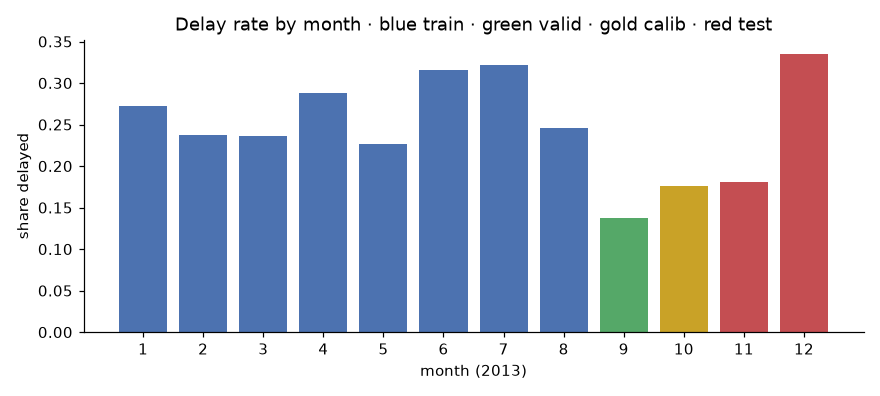
\includegraphics[width=\columnwidth]{01_split_delay_rate.png}
\caption{Delay rate by month: train (blue), valid (green), calib (gold), test (red).}\label{fig:split}\end{figure}

\subsection{Exploratory Analysis and Preprocessing}
All EDA uses the training block only. Aircraft year is missing for 17.47\% of flights, concentrated in MQ (95.1\%) and AA (69.5\%), whose tail numbers are absent from the planes table. Because this is systematic, deleting rows would bias two airlines; we impute the training median and add a missing-indicator column. 9.10\% of arrival delays are IQR outliers; they are real and cannot distort a yes/no label, so they are kept. There are 0 duplicates. The delay rate rises from 0.105 at 05:00 to 0.395 at 20:00 (delay propagation), differs more than twofold between carriers, and is lowest on Saturdays (Fig.~\ref{fig:eda}).

The daily delay rate has lag-1 autocorrelation 0.343, a PACF cut-off after lag 1 (lag-2 PACF -0.109) and lag-7 autocorrelation 0.008; the ADF test rejects a unit root ($p<10^{-10}$). Yesterday therefore carries most of the memory (a 1-day history window), and the weekly pattern is a fixed day-of-week effect (calendar features), not weekly memory. Longer 7- and 28-day windows are used only for small groups whose daily rates are noisy.

With 0.268 of training flights delayed, imbalance is moderate, so we do not re-sample (it distorts probabilities \cite{chawla2002}). Linear models get median imputation, scaling and one-hot encoding (levels with $<50$ training flights grouped); trees get ordinal codes and no scaling; XGBoost uses native categorical splits. A standard and a robust scaler tied on September (PR AUC 0.1974 vs 0.1978); the standard scaler is kept. Every statistic is fitted inside a scikit-learn pipeline on training rows only.

\begin{figure}[t]\centering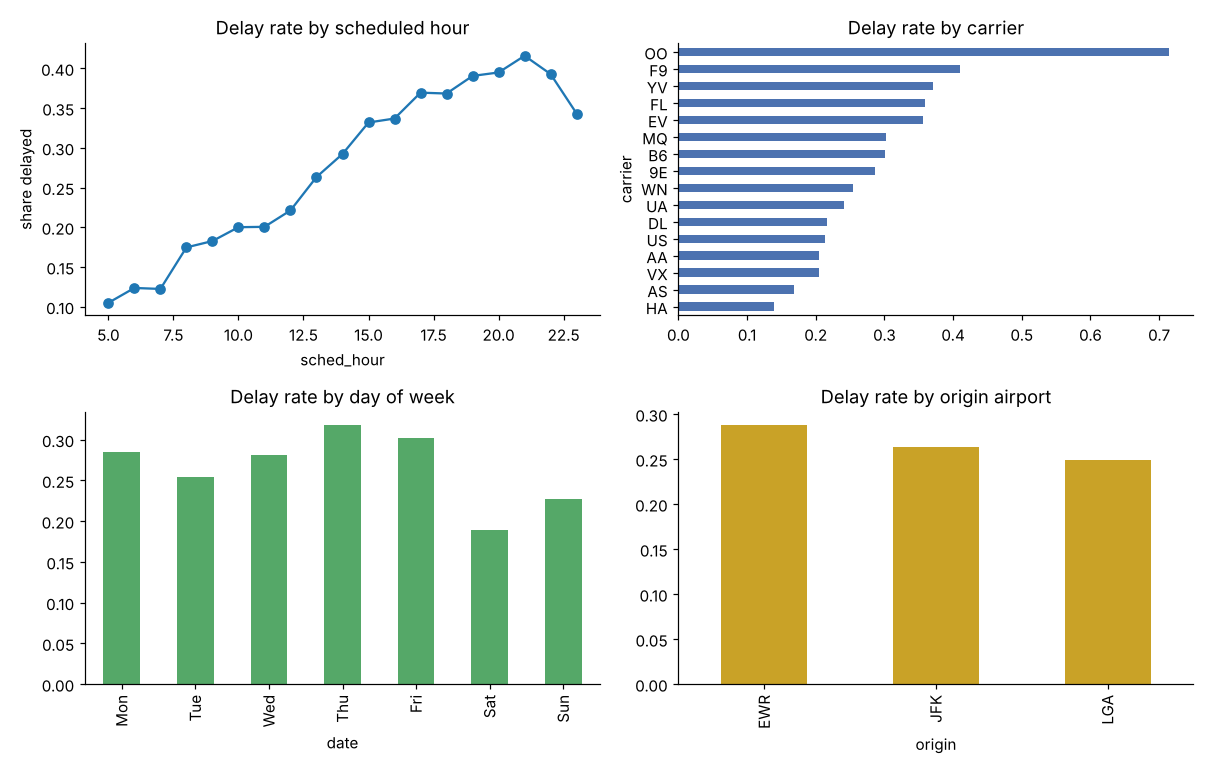
\includegraphics[width=\columnwidth]{02_delay_rate_relationships.png}
\caption{Training delay rate by hour, carrier, weekday and origin.}\label{fig:eda}\end{figure}

\section{Method}
\subsection{Leakage-Safe Features}
We build 41 numeric features in five groups plus carrier, origin and destination: cyclic (sin/cos) schedule time, calendar (day of week, weekend, days to a federal holiday), aircraft, congestion counted from the published schedule, and trailing delay history for 12 (grouping, window) pairs. History rates are shrunk towards the overall rate, $\hat r_g=(k_g+\alpha\,r_0)/(n_g+\alpha)$ with $\alpha=10$, and every grouping except all flights also gets a log-volume feature. Windows end on day D$-$1 (a rolling sum followed by a one-day shift). A unit test scrambles every outcome from a cutoff date onward and checks that features on that date are unchanged; it passes. Month and day-of-year are deliberately excluded: test months never occur in training, so they would act as date IDs.

\subsection{Models}
\textbf{Baselines.} A majority-class score, a planner's rule (the flight number's 28-day delay rate) and the scheduled hour.

\textbf{Logistic regression.} Fitted with scikit-learn as maximum-likelihood estimation of $p_i=\sigma(w^\top x_i+b)$ with an L2 penalty, inside a pipeline with the linear preprocessing above. Its inverse penalty strength $C$ is chosen on September.

\textbf{Gradient boosting.} XGBoost \cite{chen2016} adds shallow regression trees one at a time; each tree is fitted to the negative gradient of log loss, $r=y-p$, with second-order (Newton) leaf values, and a learning rate shrinks each step \cite{friedman2001}. Missing values and the three categorical columns are handled natively.

\textbf{Hybrid.} XGBoost can start from any initial prediction: with \texttt{base\_margin} set to logistic regression's logit, the trees learn only corrections, and zero trees means plain logistic regression.

\textbf{Calibration.} All learned models are Platt-scaled \cite{platt1999} on October, a month no model is fitted on.

\subsection{Evaluation Protocol}
The metric was fixed before any model: PR AUC (average precision), with ROC AUC, Brier score, expected calibration error (ECE), lift = PR AUC / base rate, and 95\% confidence intervals from a day-block bootstrap (flights on one day share weather, so days are resampled). Accuracy is rejected: predicting ``always on time'' scores 0.863 accuracy in September and catches no delays. Settings are compared on rolling months: for July, August and September, train on all earlier months and score that month. For XGBoost, early stopping must not see the scored month: for month $m$ we train on months before $m-1$, early-stop on $m-1$, refit on all months before $m$ with that many trees, and score $m$. The test months are scored once, at the end.

\section{Experiments}
\subsection{Feature Selection}
Adding groups one at a time to logistic regression, all five together score best on both September (0.261) and October (0.306). History gives the largest September gain (+0.052) but almost none in October (+0.002): which group matters depends on the month.

We tested five selection methods and adopt one only if it beats all features on \emph{both} held-out months (Table~\ref{tab:sel}). None does. Sequential forward selection reached 0.279 on September, the month it selected on, but fell to 0.281 on October against 0.306 for all features: it over-fitted its selection month. 13 features have VIF $>10$, yet pruning them lowered both months, because collinearity harms coefficient interpretation, not prediction. PCA needs 24 components for 95\% variance. All features are kept.

\begin{table}[t]\centering\caption{Feature selection (logistic regression PR AUC). None beats all features on both months.}\label{tab:sel}
\footnotesize\begin{tabular}{lrcc}\toprule
Method & $n$ & September & October\\\midrule
all features & 41 & 0.261 & 0.306\\
filter: top 10 by MI & 10 & 0.240 & 0.263\\
VIF pruning (<= 10) & 34 & 0.256 & 0.302\\
wrapper: SFS (12) & 12 & 0.279 & 0.281\\
embedded: L1, C=0.002 & 25 & 0.257 & 0.302\\
PCA (24 comps, 95\% var) & 24 & 0.268 & 0.292\\
\bottomrule\end{tabular}\end{table}

\subsection{Baselines and Model Selection}
Baselines on September / October: majority class 0.137 / 0.176; the flight number's 28-day delay rate 0.190 / 0.269; scheduled hour 0.188 / 0.229.

A short batch gradient-descent loop on the numeric features shows the effect of the learning rate: after 100 epochs, 0.01 was still slow (training log loss 0.6195), 0.5 reached 0.5282 and 8 diverged (2.3942). The L2 strength chosen on September is $C=0.001$; train and September scores hardly change with $C$, so the linear model is limited by bias, not variance. A single decision tree memorises: unlimited depth scores 1.000 on train and 0.140 on September.

Model families were compared on rolling months with fixed, untuned settings (Table~\ref{tab:family}). Mean PR AUC ranks them: logistic regression (0.408), random forest (0.386), untuned XGBoost (0.366), decision tree (0.328). Since default hyper-parameters are not a fair test of boosting, it proceeds to honest tuning.

\begin{table}[t]\centering\caption{Model families on rolling months (PR AUC, fixed settings).}\label{tab:family}
\setlength{\tabcolsep}{3pt}\footnotesize\begin{tabular}{lccccc}\toprule
Model & Jul & Aug & Sep & Mean & Fit s\\\midrule
Logistic regression & 0.557 & 0.406 & 0.262 & 0.408 & 2.6\\
Decision tree & 0.486 & 0.353 & 0.145 & 0.328 & 1.4\\
Random forest & 0.554 & 0.389 & 0.216 & 0.386 & 6.3\\
Gradient boosting (untuned) & 0.559 & 0.369 & 0.170 & 0.366 & 1.8\\
\bottomrule\end{tabular}\end{table}

\subsection{Tuning Gradient Boosting}
\textbf{The early-stopping trap.} Early-stopping on the month that is then scored lets the stopping rule see the answers. For one fixed configuration this changed the mean rolling PR AUC from 0.382 (honest protocol) to 0.402 (Table~\ref{tab:trap}).

\begin{table}[t]\centering\caption{Same configuration, two protocols (PR AUC).}\label{tab:trap}
\footnotesize\begin{tabular}{lcc}\toprule
Month & Early-stop on scored month & Honest protocol\\\midrule
Jul & 0.571 & 0.545\\
Aug & 0.392 & 0.376\\
Sep & 0.242 & 0.225\\
mean & 0.402 & 0.382\\
\bottomrule\end{tabular}\end{table}

\textbf{Random search.} 8 of 288 XGBoost configurations, each scored honestly, selected learning\_rate=0.03, max\_depth=3, min\_child\_weight=50, subsample=0.7, colsample\_bytree=0.5, reg\_lambda=1.0 (mean 0.386). All configurations lay within 0.010 of each other, all below logistic regression (0.409), and the tree count chosen by early stopping varied widely between folds ([40, 110, 13] for the best configuration). Table~\ref{tab:roll} compares the three final candidates on the same honest folds.

\begin{table}[t]\centering\caption{Rolling-month PR AUC of the final candidates.}\label{tab:roll}
\footnotesize\begin{tabular}{lcccc}\toprule
Model & Jul & Aug & Sep & Mean\\\midrule
Logistic regression & 0.556 & 0.406 & 0.266 & 0.409\\
Gradient boosting (tuned) & 0.548 & 0.391 & 0.219 & 0.386\\
Hybrid: boosting from LR & 0.559 & 0.391 & 0.268 & 0.406\\
\bottomrule\end{tabular}\end{table}

\textbf{Final training.} The tree count is the median of the fold counts: 40 for boosting and 16 for the hybrid (folds [16, 1219, 15]). Early stopping on September alone would have kept only 1 tree. All three models are refitted on January 15 -- September 30 and Platt-calibrated on October.

\section{Results}
\subsection{Test Months}
The test months were scored once (Table~\ref{tab:test}, Fig.~\ref{fig:test}). All learned models clearly beat both baselines, and the three learned models' 95\% intervals overlap heavily: the hybrid scores 0.403 and logistic regression 0.403, and boosting is 0.013 below logistic regression, well inside the interval width. Platt scaling on October lowered the calibration error of boosting (0.034 $\rightarrow$ 0.023) and raised it for logistic regression (0.029 $\rightarrow$ 0.035) and the hybrid (0.028 $\rightarrow$ 0.032). October's lower base rate pulls calibrated probabilities down, which hurts models that were already well calibrated.

\begin{table*}[t]\centering\caption{Test results, Nov--Dec 2013 (base rate 0.258). CI: 95\% day-block bootstrap. ECE: raw / after Platt.}\label{tab:test}
\footnotesize
\begin{tabular}{lcccccc}\toprule
Model & PR AUC & 95\% CI & ROC AUC & Lift & Brier & ECE raw / Platt\\\midrule
Majority class & 0.258 & -- & 0.500 & 1.00 & 0.192 & 0.010\\
Rule: flight's 28-day delay rate & 0.369 & -- & 0.638 & 1.43 & 0.184 & 0.036\\
Logistic regression & 0.403 & [0.351, 0.459] & 0.670 & 1.56 & 0.179 & 0.029 / 0.035\\
Gradient boosting & 0.390 & [0.336, 0.451] & 0.654 & 1.51 & 0.182 & 0.034 / 0.023\\
Hybrid (boosting from LR) & 0.403 & [0.352, 0.458] & 0.670 & 1.56 & 0.179 & 0.028 / 0.032\\
\bottomrule\end{tabular}\end{table*}

\begin{figure}[t]\centering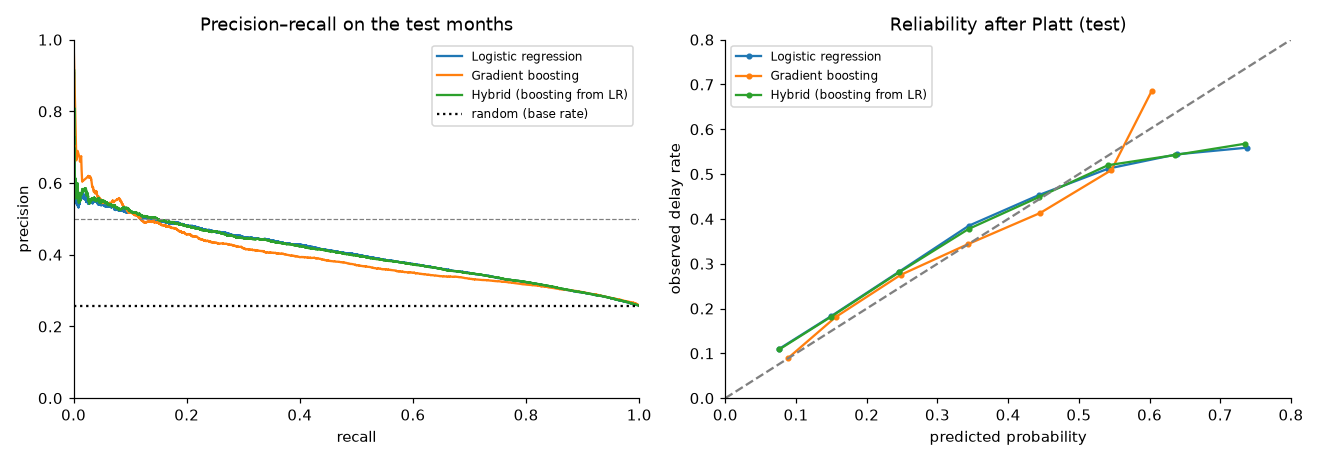
\includegraphics[width=\columnwidth]{05_test_pr_reliability.png}
\caption{Test precision--recall curves and reliability after Platt scaling.}\label{fig:test}\end{figure}

\subsection{Business Mapping}
Table~\ref{tab:biz} turns scores into a flag list per 1,000 test flights. A score threshold fixed in October, rule (a), keeps precision at 0.538--0.547 but flags only 25--26 flights and catches 0.053--0.056 of delays, because the delay rate rose from 0.176 to 0.258. Flagging when the calibrated probability is $\geq 0.5$, rule (b), keeps precision at 0.517--0.529 and flags 42--49 flights (recall 0.085--0.097), roughly twice as many true delays as a random list of the same size. Rule (b) is the policy we can state in advance.

\begin{table}[t]\centering\caption{Flag list per 1,000 test flights.}\label{tab:biz}
\setlength{\tabcolsep}{2pt}\footnotesize\begin{tabular}{llccccc}\toprule
Model & Rule & Prec. & Recall & Flagged & Delayed & Random\\\midrule
LR & (a) & 0.538 & 0.055 & 26.4 & 14.2 & 6.8\\
LR & (b) & 0.525 & 0.086 & 42.6 & 22.3 & 11.0\\
Boosting & (a) & 0.547 & 0.053 & 25.2 & 13.8 & 6.5\\
Boosting & (b) & 0.517 & 0.097 & 48.6 & 25.2 & 12.6\\
Hybrid & (a) & 0.547 & 0.056 & 26.2 & 14.4 & 6.8\\
Hybrid & (b) & 0.529 & 0.085 & 41.6 & 22.0 & 10.8\\
\bottomrule\end{tabular}\end{table}

\subsection{What Drives the Model}
Importance and ablation use October, never the test set. By permutation importance boosting relies most on scheduled hour (0.01726 drop in PR AUC) and the flight number's 28-day delay rate (0.01424). Adding feature groups to boosting one at a time, October PR AUC peaks at 0.303 with schedule, calendar and aircraft, falls to 0.291 with congestion and to 0.264 with history, while logistic regression gained from both groups. Trees split on absolute levels (for example, ``28-day rate above some cut-off'') learned in a high-delay summer; in calmer autumn months those thresholds sit in the wrong place, whereas a linear model only rescales the rate. The same drift shows by slice: boosting's lift is 1.38 in November against 1.58 for logistic regression, and December is hard for every model (about 1.35).

\begin{figure}[t]\centering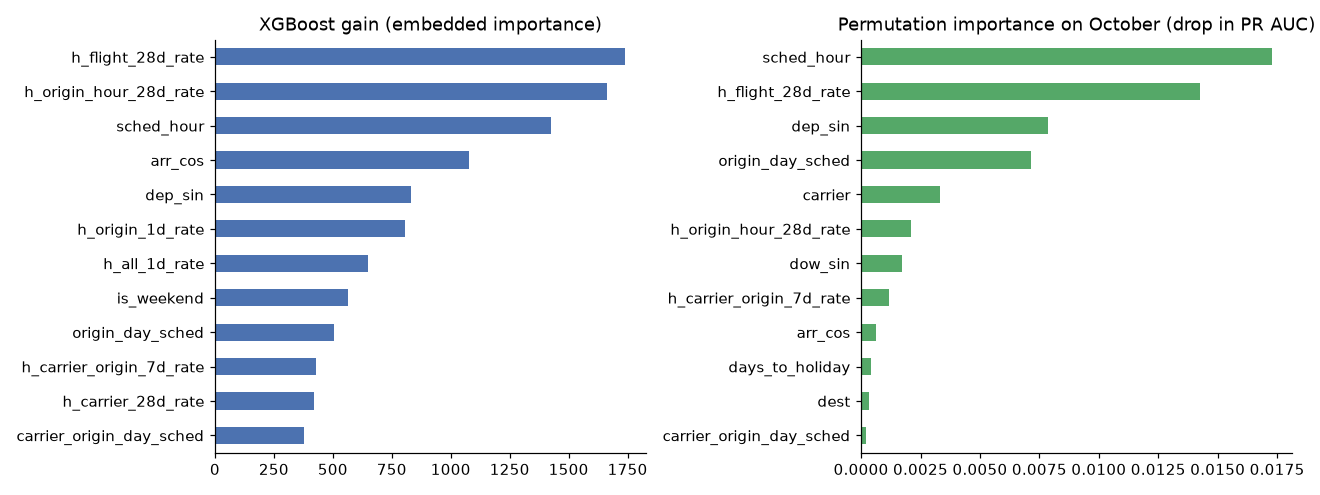
\includegraphics[width=\columnwidth]{05_importance.png}
\caption{XGBoost gain and permutation importance on October.}\label{fig:imp}\end{figure}

\subsection{Threats to Validity}
The chronological split and day-block intervals prevented an inflated or over-confident claim, the two-month veto stopped SFS from shrinking the feature set, and the honest protocol removed a 0.020 optimism from boosting's tuning score. Limitations: (i) $C=0.001$ was chosen on September and then reused in the rolling comparison whose September fold is the same month (0.2655 vs 0.2624 with $C=1$), and boosting's configuration was likewise picked on the folds it is reported on, so both rolling means are slightly optimistic; the test set is unaffected. (ii) The search covered 8 of 288 configurations, although their spread was small. (iii) The hybrid's tree counts per fold were [16, 1219, 15]; the median rule absorbs the spread, but it shows how unstable the transferable correction is. (iv) Ablation is based on one month and a fixed tree count. (v) One year of data cannot separate season from trend. (vi) All notebooks were run in order on one machine (Python 3.12.11, scikit-learn 1.9.1, XGBoost 3.4.1); other library versions may differ in the third decimal.

\section{Conclusion}
At a 05:00 decision time, gradient boosting does not significantly outperform a regularised logistic regression; both clearly beat simple baselines, and a hybrid that boosts from the linear prediction matches the linear model. The useful information at 05:00 is mostly recent delay history, which a linear model uses as well as trees and transfers better across seasons. Honest tuning matters: a common early-stopping shortcut would have overstated boosting.

\section*{Contributions}
\textbf{Shaik Junaid Sami}: problem definition, data collection, success metrics and the chronological split (notebook 01); report and presentation. \textbf{Nakkina Lakshmi Praneeth}: exploratory data analysis and preprocessing (notebook 02). \textbf{Balanagu Sesha Srikar}: feature engineering, feature selection and the leakage test (notebook 03). \textbf{Siraparapu Shiva Sankar Mani Kanta}: baselines, logistic regression and model selection (notebook 04). \textbf{Rishik Chowdary Karuturi}: gradient boosting, honest tuning, final training and test evaluation (notebook 05).

\begin{thebibliography}{99}\footnotesize
\bibitem{sternberg2017} A.~Sternberg, J.~Soares, D.~Carvalho and E.~Ogasawara, ``A review on flight delay prediction,'' arXiv:1703.06118, 2017.
\bibitem{rebollo2014} J.~J.~Rebollo and H.~Balakrishnan, ``Characterization and prediction of air traffic delays,'' \emph{Transportation Research Part C}, vol.~44, pp.~231--241, 2014.
\bibitem{gui2020} G.~Gui, F.~Liu, J.~Sun, J.~Yang, Z.~Zhou and D.~Zhao, ``Flight delay prediction based on aviation big data and machine learning,'' \emph{IEEE Trans.\ Vehicular Technology}, vol.~69, no.~1, pp.~140--150, 2020.
\bibitem{friedman2001} J.~H.~Friedman, ``Greedy function approximation: a gradient boosting machine,'' \emph{Annals of Statistics}, vol.~29, no.~5, pp.~1189--1232, 2001.
\bibitem{chen2016} T.~Chen and C.~Guestrin, ``XGBoost: a scalable tree boosting system,'' in \emph{Proc.\ ACM SIGKDD}, 2016, pp.~785--794.
\bibitem{platt1999} J.~Platt, ``Probabilistic outputs for support vector machines and comparisons to regularized likelihood methods,'' in \emph{Advances in Large Margin Classifiers}, MIT Press, 1999.
\bibitem{niculescu2005} A.~Niculescu-Mizil and R.~Caruana, ``Predicting good probabilities with supervised learning,'' in \emph{Proc.\ ICML}, 2005, pp.~625--632.
\bibitem{chawla2002} N.~V.~Chawla, K.~W.~Bowyer, L.~O.~Hall and W.~P.~Kegelmeyer, ``SMOTE: synthetic minority over-sampling technique,'' \emph{J.\ Artificial Intelligence Research}, vol.~16, pp.~321--357, 2002.
\bibitem{saito2015} T.~Saito and M.~Rehmsmeier, ``The precision-recall plot is more informative than the ROC plot when evaluating binary classifiers on imbalanced datasets,'' \emph{PLoS ONE}, vol.~10, no.~3, e0118432, 2015.
\bibitem{tashman2000} L.~J.~Tashman, ``Out-of-sample tests of forecasting accuracy: an analysis and review,'' \emph{Int.\ J.\ Forecasting}, vol.~16, no.~4, pp.~437--450, 2000.
\bibitem{kaufman2012} S.~Kaufman, S.~Rosset, C.~Perlich and O.~Stitelman, ``Leakage in data mining: formulation, detection, and avoidance,'' \emph{ACM Trans.\ Knowledge Discovery from Data}, vol.~6, no.~4, 2012.
\bibitem{kunsch1989} H.~R.~K\"unsch, ``The jackknife and the bootstrap for general stationary observations,'' \emph{Annals of Statistics}, vol.~17, no.~3, pp.~1217--1241, 1989.
\bibitem{wickham2013} H.~Wickham, \emph{nycflights13: Flights that departed NYC in 2013}, R package, 2013.
\end{thebibliography}

\onecolumn
\section*{Appendix: Decision Log}
One line per design decision (NB = notebook); the reasons are in the sections above.
\footnotesize
\begin{longtable}{@{}r c >{\raggedright\arraybackslash}p{3.0in} >{\raggedright\arraybackslash}p{3.2in}@{}}
\toprule
\# & NB & Decision & Outcome\\\midrule\endhead
1 & 01 & Binary label: arrives $\geq$15 min late & 327,346 labelled flights, 0.245 delayed\\
2 & 01 & Decision time 05:00; history ends on D$-$1; post-departure columns banned & Both leakage tests pass\\
3 & 01 & Cancelled/diverted flights unlabelled but kept on the schedule & 8,255 cancelled + 1,175 diverted not scored\\
4 & 01 & PR AUC as main metric, not accuracy & ``Always on time'' has 0.863 accuracy and zero recall\\
5 & 01 & Chronological split; test Nov--Dec used once & Monthly delay rate 0.137--0.336\\
6 & 01 & Day-block bootstrap confidence intervals & LR test PR AUC CI [0.351, 0.459]\\
7 & 02 & EDA and preprocessing statistics from training rows only & All fitted inside scikit-learn pipelines\\
8 & 02 & Impute aircraft fields + missing indicator, keep rows & 17.47\% missing, mostly MQ and AA; no rows lost\\
9 & 02 & Keep delay outliers & 9.1\% IQR outliers, all real delays\\
10 & 02 & History windows from ACF/PACF & ACF lag 1 = 0.343, lag 7 = 0.008\\
11 & 02 & No SMOTE / re-sampling & LR raw test ECE 0.029\\
12 & 02 & Standard scaler for linear models & Tie with robust scaler (0.1974 vs 0.1978)\\
13 & 03 & 41 numeric features in 5 groups + 3 categorical & All groups best: Sep 0.261, Oct 0.306\\
14 & 03 & Shrink history rates towards the overall rate ($\alpha$ = 10) & Small, noisy groups pulled to the mean\\
15 & 03 & No month or day-of-year feature & Test months never seen in training\\
16 & 03 & Keep all features unless a method wins on Sep and Oct & None did (SFS: Oct 0.281 vs 0.306)\\
17 & 04 & Baselines before any learned model & Sep PR AUC: majority 0.137, 28-day rule 0.190\\
18 & 04 & Learning-rate demo with batch gradient descent & Log loss after 100 epochs: lr 0.01 0.6195, 0.5 0.5282, 8 2.3942\\
19 & 04 & L2 strength C chosen on September only & C = 0.001\\
20 & 04 & Decision-tree depth sweep & Unlimited depth: train 1.000, Sep 0.140\\
21 & 04 & Families compared on rolling Jul/Aug/Sep, fixed settings & logistic regression 0.408 $>$ random forest 0.386 $>$ untuned XGBoost 0.366 $>$ decision tree 0.328\\
22 & 05 & Honest early stopping: stop on $m-1$, refit, score $m$ & Optimistic 0.402 vs honest 0.382\\
23 & 05 & Random search over 8 of 288 XGBoost configurations & Best mean 0.386 (LR 0.409)\\
24 & 05 & Hybrid: XGBoost starts from LR's logit & Rolling mean 0.406\\
25 & 05 & Final tree count = median of fold counts & 40 trees (September alone: 1)\\
26 & 05 & Platt calibration on October & Boosting ECE 0.034 $\rightarrow$ 0.023\\
27 & 05 & Test months scored once, all models together & PR AUC: LR 0.403, boosting 0.390, hybrid 0.403\\
28 & 05 & Flag when calibrated $p \geq 0.5$ & Precision 0.517--0.529, recall 0.085--0.097\\
29 & 05 & Importance and ablation on October, never on test & Ablation: peak 0.303, + history 0.264\\
\bottomrule
\end{longtable}
\end{document}
